\documentclass[aspectratio=169]{beamer}

% Theme settings
\usetheme{Madrid}
%\usecolortheme{beaver}
\usecolortheme{Columbia}
\setbeamertemplate{navigation symbols}{}
\setbeamertemplate{itemize items}[circle]

% Packages for Math and Graphics
\usepackage{amsmath}
\usepackage{amssymb}
\usepackage{bm} % For bold math symbols (vectors/tensors)
\usepackage{graphicx}
\usepackage{booktabs}
\usepackage{tikz}
\usepackage{pgfplots}
\pgfplotsset{compat=1.18}
\usetikzlibrary{decorations.pathmorphing,snakes,patterns}
\usepackage{hyperref} % For clickable URLs and escaping underscores via \url

% Define Draft Watermark
\newcommand{\draft}{%
    \begin{tikzpicture}[remember picture, overlay]
        \node[rotate=45, scale=8, text opacity=0.1, text=red] at (current page.center) {DRAFT!};
    \end{tikzpicture}
}

% Package for Notes
%\usepackage{pgfpages}
%\setbeameroption{show notes on second screen}

% Title Information
\title[Modern Aerospace Propulsion]{Electric Propulsion Systems}
\subtitle{Physics, Engineering, and System Integration}
\author{David Tew}
\institute{AEME \\ Columbia University}
\date{\today}

\begin{document}

%---------------------------------------------------------
% Title Slide
%---------------------------------------------------------
\begin{frame}
    \titlepage
\end{frame}

%---------------------------------------------------------
% Outline
%---------------------------------------------------------
\begin{frame}{Lecture Outline}
    \tableofcontents
\end{frame}


%---------------------------------------------------------
% Section 1: Solid Chemical Propulsion
%---------------------------------------------------------

\section{Solid Chemical Propulsion}

% --- Section 1: Introduction ---
\subsection{Introduction \& Example Propellant Chemistry}

\begin{frame}{Solid Chemical Propulsion Overview}
  \begin{block}{Solid Chemical Propulsion Systems:}
    Solid chemical propulsion offers high volumetric energy density, long-term storability, and instant readiness.  Their scale
    ranges from micro-scale thrusters for attitude control to large boosters for heavy-lift launch vehicles.
  \end{block}
  \vspace{0.5cm}
    \textbf{Critical Physics:}
    \begin{itemize}
        \item Saint-Robert's Law ($r_b=aP^n_c$) -- burning rate dependence on chamber pressure.
        \item Heterogeneous combustion physics -- with multiple reacting phases.
        \item Erosive burning regimes in high $L/D$ motors.
    \end{itemize}
\end{frame}

\begin{frame}{Example Composite Propellant ($NH_4ClO_4$/HTPB/Al)}
    \begin{columns}

        \column{0.65\textwidth}
        \textbf{Constituents \& Roles:}
        \begin{itemize}
            \item \textbf{Oxidizer:} $NH_4ClO_4$ (AP)
            \item \textbf{Binder:} HTPB. Structure + fuel source via pyrolysis.
            \item \textbf{Fuel:} Aluminum. $T_{flame} \approx 3400K$; acoustic damper.
        \end{itemize}

        \column{0.35\textwidth}
        \centering

        % TikZ Diagram: APCP Surface Structure
        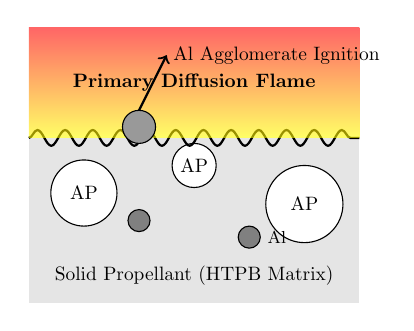
\begin{tikzpicture}[scale=0.7, transform shape]
            % Propellant Bulk
            \fill[gray!20] (0,0) rectangle (6,3);
            \node at (3,0.5) {Solid Propellant (HTPB Matrix)};
            
            % AP Crystals
            \draw[fill=white] (1,2) circle (0.6);
            \node at (1,2) {AP};
            \draw[fill=white] (3,2.5) circle (0.4);
            \node at (3,2.5) {AP};
            \draw[fill=white] (5,1.8) circle (0.7);
            \node at (5,1.8) {AP};
            
            % Al Particles
            \draw[fill=gray] (2,1.5) circle (0.2);
            \draw[fill=gray] (4,1.2) circle (0.2);
            \node at (4.5, 1.2) {\small Al};

            % Burning Surface
            \draw[thick, decorate, decoration={snake, amplitude=1mm}] (0,3) -- (6,3);
            
            % Flame Zone
            \shade[bottom color=yellow, top color=red, opacity=0.6] (0,3) rectangle (6,5);
            \node at (3, 4) {\textbf{Primary Diffusion Flame}};
            
            % Al Agglomeration
            \draw[fill=gray!80, draw=black] (2, 3.2) circle (0.3);
            \draw[->, thick] (2, 3.5) -- (2.5, 4.5);
            \node[right] at (2.5, 4.5) {Al Agglomerate Ignition};
            
        \end{tikzpicture}
    \end{columns}

        \vspace{1em}
        \textbf{Sequential Combustion Mechanism:}
        \begin{enumerate}
            \item AP phase change (orthorhombic to cubic)
            \item HTPB binder pyrolysis $\rightarrow$ gaseous HC fuels + solid char
            \item AP Decomposition: $NH_4ClO_4 \longrightarrow NH_3 + HClO_4 \longrightarrow Cl_2 + O_2 + H_2O + N_2$
            \item Surface diffusion flame
            \item Al Melting \& Combustion (far from surface).
        \end{enumerate}

\end{frame}

% --- Section 3: Internal Ballistics ---
\subsection{Internal Ballistics}

\begin{frame}{Combustion Chamber Control Volume ($V_c$) Analysis}
    \begin{itemize}
        \item Gaseous Mass Conservation:
        \begin{align*}
          \frac{d}{dt}(\rho_g V_c) &= \dot{m}_{gen} - \dot{m}_{out} \\
          V_c\frac{d\rho_g}{dt} + \rho_g \frac{dV_c}{dt} &= \dot{m}_{gen} - \dot{m}_{out}
        \end{align*}
        \item $V_c$ increases as the grain burns:
        $$\frac{dV_c}{dt} = A_b r_b$$
        \item $A_b$ is the burning surface area, and $r_b$ is the burn rate.
        \vspace{0.2em}
        \item Mass generation rate from propellant burning: $\dot{m}_{gen} = \rho_p A_b r_b$
        \vspace{0.2em}
        \item Mass outflow rate through nozzle: $\dot{m}_{out} = \frac{P_c A_t}{c^*}$
    \end{itemize}
\end{frame}

\begin{frame}{Unsteady Pressure Equation}
  \textbf{Goal:} Derive an expression for $dP_c/dt$ in terms of chamber properties and burn rate.
    \begin{align*}
        V_c\frac{d\rho_g}{dt} + \rho_g \frac{dV_c}{dt} &= \dot{m}_{gen} - \dot{m}_{out} \\
        \frac{V_c}{RT_c}\left[ \frac{dP_c}{dt} - \underbrace{\frac{P_c}{T_c}\frac{dT_c}{dt}}_{\text{Assume } \frac{dT_c}{dt}=0} \right] &= \rho_p A_b r_b - \frac{P_c A_t}{c^*} - \rho_g \frac{dV_c}{dt}\\
        \frac{dP_c}{dt} &= \frac{RT_c}{V_c} \left[ \rho_p A_b r_b \left( 1 - \frac{\rho_g}{\rho_p}\right) - \frac{P_c A_t}{c^*} \right]
    \end{align*}    
\end{frame}

\begin{frame}{Saint-Robert's Law}
  \textbf{Saint-Robert's Law:} $r_b = a P_c^n$
    \begin{itemize}
        \item $a$ = temperature dependent coefficient (hotter grains burn faster).
        \item $n$ = pressure exponent
    \end{itemize}
    \begin{columns}
                \column{0.5\textwidth}
                    \centering
                    \hspace*{1cm}% shift block right by 1 cm
                    \begin{block}{Stability Criterion ($\dot{m}_{gen} \propto P_c^n$, $\dot{m}_{out} \propto P_c$)}
              $$\begin{cases}
                  n < 1 & \text{Stable}: \uparrow P_c \Rightarrow |\Delta\dot{m}_{gen}| < |\Delta\dot{m}_{out}| \\
                  n > 1 & \text{Unstable}: \uparrow P_c \Rightarrow |\Delta\dot{m}_{gen}| > |\Delta\dot{m}_{out}|
              \end{cases}$$
          \end{block}
        \column{0.5\textwidth}
            \centering
            \begin{tikzpicture}[scale=0.6]
                \begin{axis}[
                    width=0.95\linewidth,
                    axis lines=left,
                    xlabel={$time$},
                    ylabel={$P_c$},
                    xtick=\empty, ytick=\empty,
                    xmin=0, xmax=10,
                    ymin=0,
                    clip=false
                ]
                    \addplot[domain=0:10, thick, blue] {2*x^0.5};
                    \node at (axis cs: 6, 4) [right, blue] {Stable ($n<1$)};
                    \addplot[domain=0.1:4, thick, red, dashed] {0.5*x^2};
                    \node at (axis cs: 3, 8) [right, red] {Unstable ($n>1$)};
                \end{axis}
            \end{tikzpicture}
    \end{columns}
\end{frame}

\begin{frame}{Steady State Chamber Pressure}
  \begin{itemize}
    \item \textbf{Assume Steady State:} 
    $$\frac{dP_c}{dt} = 0$$
    $$\rho_p A_b r_b \left( 1 - \underbrace{\frac{\rho_g}{\rho_p}}_{neglect}\right) = \frac{P_c A_t}{c^*}$$
    \item \textbf{Substitute Saint-Robert's Law ($r_b = a P_c^n$):}
          $$\rho_p A_b a P_c^n = \frac{P_c A_t}{c^*}$$
    \item \textbf{Equilibrium Pressure:}
          $$P_{c}^{eq} \approx \left[ \rho_p a c^* K_n \right]^{\frac{1}{1-n}}$$
          \item Note sensitivity to $K_n = A_b / A_t$. If $n=0.5$, $P \propto K_n^2$.
  \end{itemize}
\end{frame}

% --- Section 4: Grain Design ---
\subsection{Grain Design}

\begin{frame}{Burn Area ($A_b$) Geometric Evolution}
  \textbf{Evolution of Grain Geometry ($A_b(t)$) Controls Thrust Profile:}
    \begin{itemize}
        \item \textbf{Progressive:} $A_b$ increases $\Rightarrow$ $T$ increases.
        \item \textbf{Neutral:} $A_b$ constant $\Rightarrow$ $T$ constant.
        \item \textbf{Regressive:} $A_b$ decreases $\Rightarrow$ $T$ decreases.
    \end{itemize}
    \vspace{1em}
    \textbf{Common Grain Geometries:}
    \begin{itemize}
        \item \textbf{Progressive:}Circular Perforation or Center-Perforated Cylinder
        \item \textbf{Neutral:} Star or Wagon Wheel
        \item \textbf{Regressive:} Outer-burning grains or multi-propellant stacks
    \end{itemize}
\end{frame}

\begin{frame}{Advanced Grain Geometries: Star and Finocyl}
    \begin{columns}
        \column{0.5\textwidth}
        \textbf{Star:}
        \begin{itemize}
            \item $A_b \approx $ constant (neutral burn). 
            \item Sliver formation an efficiency challenge.
        \end{itemize}
        \vspace{1em}

        \centering
        % TikZ: Grain Cross Sections
        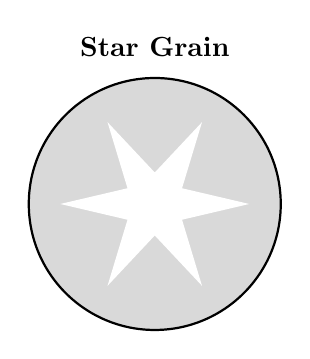
\begin{tikzpicture}[scale=0.8]
          % Star Grain
          \node at (0, 2.5) {\textbf{Star Grain}};
          \draw[thick, fill=gray!30] (0,0) circle (2);
          % Six-pointed star (centered), alternating outer/inner radii
          \fill[white] (0:1.5) -- (30:0.5) -- (60:1.5) -- (90:0.5) -- (120:1.5) -- (150:0.5)
                       -- (180:1.5) -- (210:0.5) -- (240:1.5) -- (270:0.5) -- (300:1.5) -- (330:0.5) -- cycle;
          
          % Web Definition
          %\draw[red, <->] (60:1.5) -- (60:2);
          %\node[red, right] at (60:1.8) {Web ($w$)};
        \end{tikzpicture}

        \column{0.5\textwidth}
        \textbf{Finocyl (Fin-On-Cylinder):}
        \begin{itemize}
            \item Provides flexibility in thrust profile design.
            \item Shuttle SRM: High thrust after launch, lower thrust during max-Q.
        \end{itemize}

        % Use \url to safely typeset underscores in the link
        \note{\url{https://wikis.mit.edu/confluence/display/RocketTeam/Commercial+Grain+Geometries}}

        \centering
        % TikZ: Grain Cross Sections
        % External Finocyl Image (replace placeholder path with your figure)
        % If the image file exists at figs/finocyl.png it will be included;
        % otherwise a framed placeholder box will appear as a reminder.
        \IfFileExists{figs/Shuttle\_SRB.jpg}{%
            \includegraphics[width=0.9\linewidth]{figs/Shuttle\_SRB.jpg}%
        }{%
            \fbox{\parbox{0.9\linewidth}{Finocyl image placeholder\\Add image at figs/Shuttle\_SRB.jpg}}%
        }
    \end{columns}
\end{frame}

\begin{frame}{Burnback Analysis \& Optimization}
  \textbf{Goal:} Optimize $A_b(t=0)$ to provide the $A_b(t)$ that enables the target thrust profile.
    \begin{itemize}
        \item \textbf{Analytical Methods:} Simplified geometries (cylinders, stars) allow closed-form $A_b(t)$ expressions.
        \item \textbf{Level Set Methods:}: Implicit surface tracking via signed distance functions.
        $$\phi(x,y,t) = \begin{cases}
            >0 & \text{in solid} \\
            =0 & \text{on surface} \\
            <0 & \text{in gas}
        \end{cases}$$
        $$\frac{\partial \phi}{\partial t} + r_b |\nabla \phi| = 0$$
        \item \textbf{Optimization:} Iterate on initial geometry to achieve desired $A_b(t)$ and thrust profile.
    \end{itemize}

\end{frame}

% --- Section 5: Flow Physics ---
\subsection{Flow Physics \& Erosion}

\begin{frame}{Erosive Burning \& Velocity Coupling}
  \draft
  \textbf{Phenomenon:} 
  \begin{itemize}
    \item Stagnant chamber assumption fails in high $L/D$ motors.
    \item High velocity ($u$) enhances heat transfer to the propellant, increasing burn rate beyond Saint-Robert's prediction.
  \end{itemize}
  
  \begin{block}{Lenoir-Robillard Model}
      $$r_{total} = r_{base} + r_{erosive}$$
      $$r_{base} = a P_c^n$$
      $$r_{erosive} = \alpha G^{0.8} L^{-0.2} e^{-\beta r_{total} \rho_p / G}$$
      \centering
      where $G = \rho_g u$ is the mass flux; $\alpha, \beta$ are empirical constants.
  \end{block}
  

\end{frame}

\begin{frame}{Implications of Erosive Burning}
  \begin{block}{System Implications:}
    Erosive burning typically occurs in high $L/D$ motors immediately after ignition when $u$ is highest. 
    As the grain burns, the port area ($A_{port}$) opens, reducing $u$ and thus erosive effects.
  \end{block}
  \begin{block}{Negative Erosion:}
    In some geometries, high velocity can cool the surface and slow the burning rate.
  \end{block}
\end{frame}

% --- Section 6: Instability ---
\subsection{Combustion Instability}

\begin{frame}{Acoustic Instability: Hart-McClure Criterion}
  \begin{alertblock}{Combustion Instability}
    Acoustic eigenmodes in the chamber can couple with unsteady heat release from the burning propellant, 
    leading to large pressure oscillations or DC pressure increases that can damage or destroy the motor.
  \end{alertblock}

    \textbf{Stability:} Determined by the net growth rate $\alpha_{net}$.
    $$\alpha_{net} = \underbrace{\alpha_{pressure} + \alpha_{velocity}}_{\text{Gains (Driving)}} - \underbrace{(\alpha_{nozzle} + \alpha_{particle} + \alpha_{wall})}_{\text{Losses (Damping)}} $$
    $$\alpha_{net} < 0 \Rightarrow \text{Stable}; \quad \alpha_{net} > 0 \Rightarrow \text{Unstable}$$

    \begin{itemize}
        \item \textbf{Pressure Coupling:} Increased surface pressures can accelerate burning.
        \item \textbf{Particle Damping:} $Al_2O_3$ droplets lag gas oscil. \& dissipate energy via viscous drag.
        \item \textbf{Design Trade-off:} "Smokeless" missiles (no Al) lose particle damping (stability risk).
    \end{itemize}

\end{frame}

% --- Section 7: Materials ---
\subsection{Thermal Protection Systems}

\begin{frame}{Ablative Nozzle Throat Erosion \& Cooling}
  \begin{alertblock}{Nozzle Cooling Challenge}
    \begin{itemize}
      \item Combustion gas temperature ($3400K$) exceeds melting point of all metals. 
      \item Active cooling impractical due to solid grain geometry.
    \end{itemize}
  \end{alertblock}
  \vspace{0.5cm}
  \begin{columns}
    \column{0.65\textwidth}
    \textbf{Solution: Carbon-Carbon (C/C) Ablation}
    \begin{itemize}
        \item Mechanism is chemical erosion, not melting.
        \item Diffusion-controlled oxidation by $H_2O$ and $CO_2$.
        \item $C_{(s)} + H_2O_{(g)} \rightarrow CO_{(g)} + H_2$
    \end{itemize}
    \vspace{0.5cm}
    \textbf{Bartz Correlation Scaling:} $\dot{r}_{erosion} \propto P_c^{0.8} D_t^{-0.2}$

    \column{0.35\textwidth}
    % TikZ: Nozzle Ablation
    \centering
    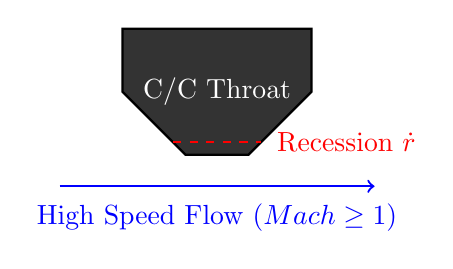
\begin{tikzpicture}[scale=0.8]
        % Nozzle Wall Initial
        \draw[thick, fill=black!80] (0,0) -- (1, -1) -- (2, -1) -- (3, 0) -- (3, 1) -- (0, 1) -- cycle;
        \node[white] at (1.5, 0) {C/C Throat};
        
        % Erodable layer
        \draw[dashed, red, thick] (0.8, -0.8) -- (2.2, -0.8);
        \node[red, anchor=west] at (2.3, -0.8) {Recession $\dot{r}$};
        
        % Gas Flow
        \draw[blue, thick, ->] (-1, -1.5) -- (4, -1.5);
        \node[blue] at (1.5, -2) {High Speed Flow ($Mach\ge1$)};
    \end{tikzpicture}
  \end{columns}

\end{frame}

% --- Conclusion ---
\subsection{Summary}
\begin{frame}{Solid Propulsion Summary}
    \begin{block}{Takeaways}
    \begin{enumerate}
        \item \textbf{Chemistry is Destiny:} APCP formulation dictates energy density and fundamental burn rate.
        \item \textbf{Geometry is Control:} 3D grain design (Finocyl/Star) determines the thrust profile ($P \propto K_n^{1/(1-n)}$).
        \item \textbf{Stability is Critical:} Acoustic eigenmodes must be damped by particles or mechanical resonators to prevent catastrophic failure.
        \item \textbf{Materials Limit Performance:} Nozzle erosion imposes limits on pressure and burn time.
    \end{enumerate}
    \end{block}
\end{frame}



\section{Electric Propulsion}
%---------------------------------------------------------
% Section 1: Introduction & Physics
%---------------------------------------------------------
\subsection{Introduction to Electric Propulsion}

\begin{frame}{Lecture Outline}
  \tableofcontents[currentsection]
\end{frame}

\begin{frame}{Chemical to Electric Propulsion}
    \begin{block}{Chemical Propulsion:}
      \begin{itemize}
          \item Energy source -- reacting fuel and oxidizer -- is the propellant.
          \item Max $v_e \approx 4.5$ km/s ($H_2/O_2$).
      \end{itemize}
    \end{block}
    \vspace{0.5cm}
    \begin{block}{Electric Propulsion:}
      \begin{itemize}
          \item Energy source decoupled from propellant.
          \item $v_e > 30$ km/s  achievable.
          \item At fixed power, $I_{sp}$ and thrust are inversely related.
      \end{itemize}
    \end{block}
\end{frame}

\begin{frame}{The Power-Limited Rocket Equation}
    Thrust ($T$) is the momentum flux of the beam:
    \begin{equation}
        T = \dot{m} v_e
    \end{equation}

    The Jet Power ($P_{jet}$) is the kinetic energy flux of the beam:
    \begin{equation}
        P_{jet} = \frac{1}{2} \dot{m} v_e^2 = \frac{1}{2} T v_e
    \end{equation}
    
    The overall efficiency is given by $\eta_T = P_{jet} / P_{in}$:
    \begin{equation}
        T = \frac{2 \eta_T P_{in}}{v_e} = \frac{2 \eta_T P_{in}}{g_0 I_{sp}}
    \end{equation}
    
    \begin{itemize}
        \item Thrust ($T$) is \textit{inversely proportional} to Specific Impulse ($I_{sp}$) @ fixed power ($P_{in}$).
        \item \textbf{Design Trade:} Minimize propellant mass (high $I_{sp}$) vs. Minimize trip time (high Thrust).
    \end{itemize}
\end{frame}

\begin{frame}{Efficiency Drivers}
    Diagnosing performance requires breaking down $\eta_T$:
    
    \begin{equation}
        \eta_T = \eta_e \cdot \eta_m \cdot \eta_b \cdot \eta_v \cdot \alpha
    \end{equation}
    
    \begin{itemize}
        \item \textbf{Electrical Efficiency ($\eta_e$):} Beam power vs. Total power (losses in magnets, heater, PPU).
        \item \textbf{Mass Utilization ($\eta_m$):} Fraction of propellant ionized ($\dot{m}_{ion} / \dot{m}_{total}$).
        \item \textbf{Beam Divergence ($\eta_b$ or $\eta_{div}$):} Loss due to plume spread ($\langle \cos \theta \rangle^2$).
        \item \textbf{Voltage Utilization ($\eta_v$):} Effective beam voltage vs. Discharge voltage ($V_b / V_d$).
        \item \textbf{Doubles Correction ($\alpha$):} Thrust loss due to multiply charged ions ($Xe^{++}$).
    \end{itemize}
\end{frame}

%---------------------------------------------------------
% Slide 1: Comparative Table
%---------------------------------------------------------
\begin{frame}{Comparative Analysis of Electric Propulsion Systems}
    \centering
    \resizebox{\textwidth}{!}{%
    \begin{tabular}{l c c c c c p{3.5cm} p{3.5cm}}
        \toprule
        \textbf{Technology} & \textbf{$I_{sp}$ (s)} & \textbf{Thrust} & \textbf{$\eta_T$} & \textbf{Power} & \textbf{TRL} & \textbf{Key Pros} & \textbf{Key Cons} \\
        \midrule
        \textbf{Resistojet} & 280--350 & 10mN--0.5N & 65--80\% & $<1$ kW & 9 & Simple; Low cost; Shared propellant & Material thermal limits; Low $I_{sp}$ \\
        \midrule
        \textbf{Arcjet} & 450--600 & 0.1N--2N & 30--45\% & 0.5--2 kW & 9 & Robust; Higher $I_{sp}$ than resistojet & Electrode erosion; Frozen flow losses \\
        \midrule
        \textbf{Gridded Ion} & 2500--4000+ & 20--250mN & 60--80\% & 0.5--7 kW & 9 & Highest Efficiency; Longest Life & Low thrust density (Grid limits); Complex PPU \\
        \midrule
        \textbf{Hall Effect} & 1500--3000 & 40mN--1N+ & 50--65\% & 0.2--20 kW & 9 & High Thrust-to-Power; Compact & Beam divergence; Channel erosion (if unshielded) \\
        \midrule
        \textbf{Electrospray} & 1000--6000 & $\mu$N--mN & $>70\%$ & mW--50W & 6--9 & Precision control; Scalable arrays & Very low thrust; High voltage; Clogging risks \\
        \midrule
        \textbf{PPT} & 800--1500 & $\mu$N-s & 5--15\% & $<100$ W & 9 & Solid fuel (Teflon); Simple storage & Very low efficiency; Carbon contamination \\
        \midrule
        \textbf{MPD} & 2000--10000 & 1N--100N & 30--60\% & MW Class & 4--5 & High thrust density at high $I_{sp}$ & Requires MW power; Cathode erosion severe \\
        \bottomrule
    \end{tabular}%
    }
\end{frame}

\begin{frame}{Designer's Guide to Thruster Selection (1 of 2)}

    \textbf{1. Is Power the Primary Constraint?}
    \begin{itemize}
        \item \textbf{Selection:} \textcolor{blue}{Hall Effect Thruster}
        \item \textit{Rationale:} Offers higher Thrust-to-Power ratio (60--80 mN/kW) than Ion engines. Reduces maneuver time for power-limited commercial satellites.
    \end{itemize}
    \vspace{0.2cm}
    
    \textbf{2. Is Propellant Mass the Primary Constraint?}
    \begin{itemize}
        \item \textbf{Selection:} \textcolor{blue}{Gridded Ion Thruster}
        \item \textit{Rationale:} Maximizes Specific Impulse ($I_{sp} > 3000$ s). Essential for high-$\Delta v$ deep space missions (e.g., Dawn, BepiColombo) to minimize launch mass.
    \end{itemize}
    \vspace{0.2cm}
    
\end{frame}

\begin{frame}{Designer's Guide to Thruster Selection (2 of 2)}
    
  \textbf{3. Is Cost or Volume Constrained?}
    \begin{itemize}
        \item \textbf{Selection:} \textcolor{blue}{Argon Hall} (Cost) or \textcolor{blue}{Iodine Hall} (Volume)
        \item \textit{Rationale:} Argon is abundant and cheap for constellations (Starlink). Iodine stores as a dense solid, eliminating high-pressure tanks for CubeSats.
    \end{itemize}
    \vspace{0.2cm}
    
    \textbf{4. Is Precision Pointing Required?}
    \begin{itemize}
        \item \textbf{Selection:} \textcolor{blue}{FEEP / Electrospray}
        \item \textit{Rationale:} Provides $\mu$N thrust resolution with no moving parts (valves). Critical for drag-free science missions (e.g., LISA).
    \end{itemize}

\end{frame}

%---------------------------------------------------------
% Section 2: Electrothermal Systems
%---------------------------------------------------------
\subsection{Electrothermal Propulsion}

\begin{frame}{Resistojets \& Arcjets}
    \textbf{Resistojets:}
    \begin{itemize}
        \item Mechanism: Gas flows over electrically heated element (Re, W).
        \item Limit: Material melting point.
        \item Performance: $I_{sp} \approx 300$ s (Hydrazine).
        \item Application: Station-keeping, attitude control.
    \end{itemize}
    
    \textbf{Arcjets:}
    \begin{itemize}
        \item Mechanism: High-current arc heats gas core $>10{,}000$ K.
        \item Physics: Cool boundary layer protects nozzle walls.
        \item Performance: $I_{sp} \approx 500-600$ s.
        \item Limitation: Electrode erosion, high power density required.
    \end{itemize}
\end{frame}

\begin{frame}{Arcjet Thruster}
  \begin{figure}[h]
  \centering
  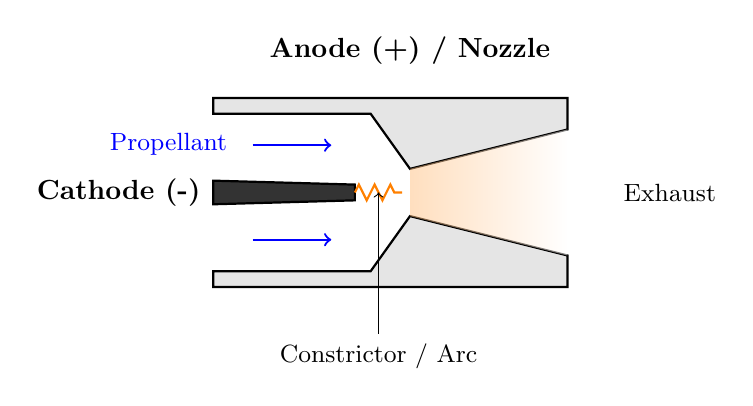
\begin{tikzpicture}
    % Nozzle / Anode (Cutaway)
    \draw[thick, fill=gray!20] (0,1) -- (2,1) -- (2.5,0.3) -- (4.5,0.8) -- (4.5,1.2) -- (0,1.2) -- cycle;
    \draw[thick, fill=gray!20] (0,-1) -- (2,-1) -- (2.5,-0.3) -- (4.5,-0.8) -- (4.5,-1.2) -- (0,-1.2) -- cycle;
    
    % Cathode Rod
    \draw[thick, fill=black!80] (0,0.15) -- (1.8,0.1) -- (1.8,-0.1) -- (0,-0.15) -- cycle;
    
    % Arc
    \draw[thick, orange, decorate, decoration={zigzag, segment length=2mm, amplitude=1mm}] (1.8,0) -- (2.4,0);
    
    % Propellant Flow
    \draw[->, blue, thick] (0.5, 0.6) -- (1.5, 0.6);
    \draw[->, blue, thick] (0.5, -0.6) -- (1.5, -0.6);
    
    % Plume
    \shade[left color=orange!50, right color=white, opacity=0.5] (2.5,0.3) -- (4.5, 0.8) -- (4.5, -0.8) -- (2.5,-0.3) -- cycle;
    
    % Labels - positioned outside/around the figure
    \node at (-1.2, 0) {\textbf{Cathode (-)}};
    \node at (2.5, 1.8) {\textbf{Anode (+) / Nozzle}};
    \draw[<-] (2.1, 0) -- (2.1, -1.8) node[below] {\small Constrictor / Arc};
    \node at (0.3, 0.35) [blue, above left] {\small Propellant};
    \node at (5.8, 0) {\small Exhaust};

  \end{tikzpicture}
  \caption{Arcjet Thruster Schematic}
  \end{figure}
\end{frame}

%---------------------------------------------------------
% Section 3: Gridded Ion Thrusters (GIT)
%---------------------------------------------------------
\subsection{Electrostatic I: Gridded Ion Thrusters}

\begin{frame}{Gridded Ion Thruster Architecture}
    \begin{columns}
        \column{0.5\textwidth}
        \textbf{Core Concept:}
        \begin{itemize}
            \item Decoupled ionization and acceleration.
            \item Highest efficiency EP device.
        \end{itemize}
        \vspace{0.2cm}
        \textbf{Ionization Generation:}
        \begin{itemize}
            \item \textbf{DC (Kaufman):} Hollow cathode + Ring-cusp magnetic confinement.
            \item \textbf{RF (RIT):} Inductive coil, electrodeless discharge (longer life).
        \end{itemize}
        
        \column{0.5\textwidth}
        \textbf{Acceleration:}
        \begin{itemize}
            \item Multi-grid assembly (Screen + Accel).
            \item Electrostatic field extracts ions.
        \end{itemize}
    \end{columns}
\end{frame}

\begin{frame}{Gridded Ion Thruster Schematic}

  \begin{figure}[h]
    \centering
    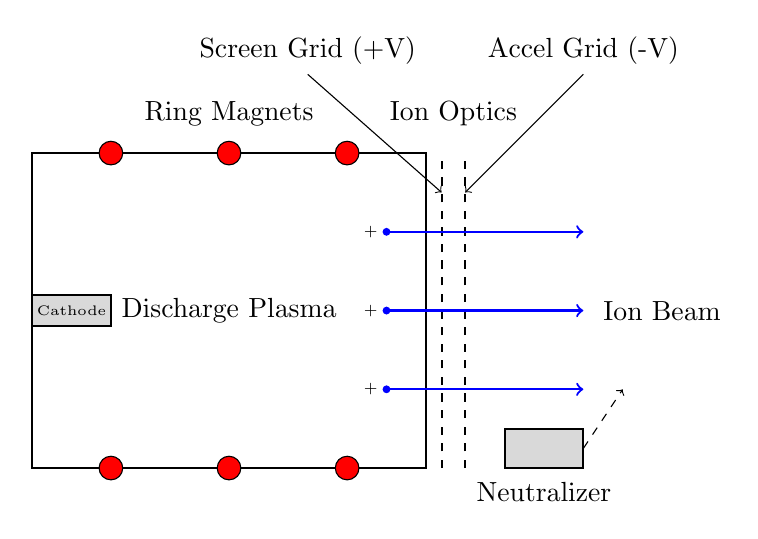
\begin{tikzpicture}
        % Discharge Chamber
        \draw[thick] (0,0) rectangle (5, 4);
        
        % Hollow Cathode
        \draw[thick, fill=gray!30] (0, 1.8) rectangle (1, 2.2);
        \node at (0.5, 2) {\tiny Cathode};
        
        % Magnetic Rings (Cusps)
        \foreach \x in {1, 2.5, 4} {
            \draw[fill=red] (\x, 4) circle (0.15);
            \draw[fill=red] (\x, 0) circle (0.15);
        }
        \node at (2.5, 4.5) {Ring Magnets};
        
        % Grids
        \draw[thick, dashed] (5.2, 0) -- (5.2, 4);
        \draw[thick, dashed] (5.5, 0) -- (5.5, 4);
        \node at (5.35, 4.5) {Ion Optics};
        \draw[<-] (5.2, 3.5) -- (3.5, 5) node[above] {Screen Grid (+V)};
        \draw[<-] (5.5, 3.5) -- (7.0, 5) node[above] {Accel Grid (-V)};
        
        % Neutralizer
        \draw[thick, fill=gray!30] (6, 0) rectangle (7, 0.5);
        \node at (6.5, -0.3) {Neutralizer};
        \draw[->, dashed] (7, 0.25) -- (7.5, 1);
        
        % Ions
        \foreach \y in {1, 2, 3} {
            \draw[->, blue, thick] (4.5, \y) -- (7, \y);
            \fill[blue] (4.5, \y) circle (0.05);
            \node at (4.3, \y) {\tiny +};
        }
        \node at (8.0, 2) {Ion Beam};
        \node at (2.5, 2) {Discharge Plasma};

    \end{tikzpicture}
    \caption{Electrostatic: Gridded Ion Thruster}

  \end{figure}

\end{frame}

\begin{frame}{The Child-Langmuir Limit}
    Thrust density is limited by space charge shielding between grids:
    
    \begin{equation}
        J_{CL} = \frac{4 \epsilon_0}{9} \sqrt{\frac{2q}{m_i}} \frac{V_T^{3/2}}{d^2}
    \end{equation}
    
    \begin{itemize}
        \item $J$: Current density ($A/m^2$)
        \item $V_T$: Total voltage ($V_{beam} + |V_{accel}|$)
        \item $d$: Grid gap
    \end{itemize}
    
    \textbf{Implication:} To increase thrust, you must increase voltage or decrease grid gap (manufacturing limit). Ion thrusters are "large" for their thrust.
\end{frame}

\begin{frame}{Optics Lifetime: Erosion Physics}
    \textbf{Primary Failure Mode: Accelerator Grid Erosion}
    \begin{itemize}
        \item Mechanism: Charge Exchange (CEX) Collisions.
        \item Fast Ion + Slow Neutral $\rightarrow$ Fast Neutral + Slow Ion.
        \item Slow ions form in the gap/plume and accelerate into the negative Accel Grid.
        \item Result: "Pits and Grooves" erosion.
    \end{itemize}
    \vspace{0.5cm}
    \textbf{Perveance Matching:}
    \begin{itemize}
        \item \textbf{Over-perveance:} Sheath bulges, direct impingement.
        \item \textbf{Under-perveance:} Beam focuses too sharply, CEX crossover.
    \end{itemize}
\end{frame}

%---------------------------------------------------------
% Section 4: Hall Effect Thrusters (HET)
%---------------------------------------------------------
\subsection{Electrostatic II: Hall Effect Thrusters}

\begin{frame}{Hall Thruster Operating Principle}
    \textbf{Cross-Field ($E \times B$) Discharge:}
    \begin{itemize}
        \item Radial Magnetic Field ($B_r$) + Axial Electric Field ($E_z$).
        \item Electrons are magnetized ($\Omega_e \gg 1$), Ions are un-magnetized.
    \end{itemize}
    
    \begin{equation}
        \Omega_e = \frac{eB}{m_e \nu_{coll}}
    \end{equation}
    
    \textbf{Magnetic Insulation:}
    \begin{itemize}
        \item High impedance to electron flow allows supporting large potential drop ($V_d \approx 300-600$ V) in a quasi-neutral plasma.
        \item \textbf{Advantage:} No Space Charge Limit! Higher thrust density than Ion Thrusters.
    \end{itemize}
\end{frame}

\begin{frame}{Hall Effect Thuster Schematic}

  \begin{figure}[h]
    \centering
    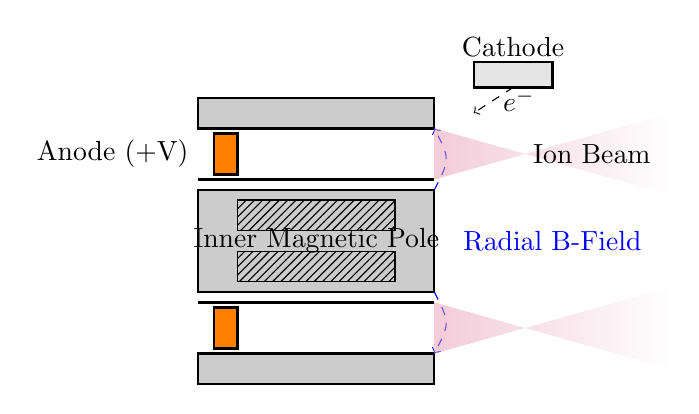
\begin{tikzpicture}[yscale=0.65]
        % Central Core (Inner Pole)
        \draw[thick, fill=gray!40] (0, -1) rectangle (3, 1);
        \node at (1.5, 0) {Inner Magnetic Pole};
        
        % Inner Coil
        \draw[pattern=north east lines] (0.5, 0.2) rectangle (2.5, 0.8);
        \draw[pattern=north east lines] (0.5, -0.8) rectangle (2.5, -0.2);
        
        % Discharge Channel Walls
        \draw[thick] (3, 1.2) -- (0, 1.2); % Inner wall top
        \draw[thick] (3, 2.2) -- (0, 2.2); % Outer wall top
        
        \draw[thick] (3, -1.2) -- (0, -1.2); % Inner wall bottom
        \draw[thick] (3, -2.2) -- (0, -2.2); % Outer wall bottom
        
        % Outer Pole
        \draw[thick, fill=gray!40] (0, 2.2) -- (3, 2.2) -- (3, 2.8) -- (0, 2.8) -- cycle;
        \draw[thick, fill=gray!40] (0, -2.2) -- (3, -2.2) -- (3, -2.8) -- (0, -2.8) -- cycle;
        
        % Anode / Gas Distributor
        \draw[thick, fill=orange] (0.2, 1.3) rectangle (0.5, 2.1);
        \draw[thick, fill=orange] (0.2, -1.3) rectangle (0.5, -2.1);
        \node at (0, 1.7) [left] {Anode (+V)};
        
        % Magnetic Field Lines (Radial)
        \draw[blue, dashed, ->] (3, 1).. controls (3.2, 1.6).. (3, 2.2);
        \draw[blue, dashed, ->] (3, -1).. controls (3.2, -1.6).. (3, -2.2);
        \node at (4.5, 0) [blue] {Radial B-Field};
        
        % Cathode
        \draw[thick, fill=gray!20] (3.5, 3) rectangle (4.5, 3.5);
        \node at (4, 3.8) {Cathode};
        \draw[->, dashed] (4, 3) -- (3.5, 2.5) node[midway, right] {$e^-$};
        
        % Beam
        \shade[left color=purple!40, right color=white, opacity=0.5] (3, 1.2) -- (6, 2.5) -- (6, 0.9) -- (3, 2.2) -- cycle;
        \shade[left color=purple!40, right color=white, opacity=0.5] (3, -1.2) -- (6, -2.5) -- (6, -0.9) -- (3, -2.2) -- cycle;
        
        \node at (5, 1.7) {Ion Beam};

    \end{tikzpicture}
    \caption{Electrostatic: Hall Effect Thruster (Cross Section)}
  \end{figure}

\end{frame}

\begin{frame}{Anomalous Transport \& Instabilities}
    \textbf{Anomalous Transport:}
    \begin{itemize}
        \item Classical collision theory predicts current $100\times$ lower than observed.
        \item Real transport driven by:
        \begin{itemize}
            \item Plasma turbulence/waves (Bohm diffusion).
            \item Near-Wall Conductivity (Secondary electron emission).
        \end{itemize}
    \end{itemize}
    \vspace{0.2cm}
    \textbf{Breathing Mode Instability (10-30 kHz):}
    \begin{itemize}
        \item "Predator-Prey" cycle between Neutrals and Ions.
        \item Ionization depletes neutrals $\rightarrow$ Current drops $\rightarrow$ Neutrals refill $\rightarrow$ Current spikes.
        \item Requires active filtering in PPU.
    \end{itemize}
\end{frame}

\begin{frame}{The Revolution: Magnetic Shielding}
    \textbf{The Problem (Pre-2010):}
    \begin{itemize}
        \item Field lines intersected ceramic walls. High energy ions eroded channel.
        \item Lifetime limit: $\approx 5,000$ hours.
    \end{itemize}
    \vspace{0.2cm}
    \textbf{The Solution (Magnetic Shielding):}
    \begin{itemize}
        \item Topology shaping: Field lines parallel to walls, grazing the anode.
        \item Creates equipotential zone near wall ($T_e$ is low).
        \item Potential drop < Sputtering threshold.
        \item \textbf{Result:} Erosion reduced $100-1000\times$. Lifetimes $>50{,}000$ hours (e.g., AEPS for Lunar Gateway).
    \end{itemize}
\end{frame}

%---------------------------------------------------------
% Section 5: Electromagnetic & Propellants
%---------------------------------------------------------
\subsection{Electromagnetic Systems \& Propellant Economics}

\begin{frame}{Electromagnetic Propulsion}
    \textbf{Lorentz Force:} $\vec{F} = \vec{J} \times \vec{B}$
    \vspace{0.5cm}
    \begin{itemize}
        \item \textbf{MPD (Magnetoplasmadynamic):} 
            \begin{itemize}
                \item Multi-MW power handling.
                \item Self-field or Applied-field.
                \item Issue: Cathode erosion at kA currents.
            \end{itemize}
        \item \textbf{PPT (Pulsed Plasma Thruster):}
            \begin{itemize}
                \item Solid Teflon ablation. Simple, robust.
                \item Low efficiency, used for CubeSats/Attitude control.
            \end{itemize}
        \item \textbf{VASIMR:}
            \begin{itemize}
                \item RF Ionization (Helicon) + RF Heating (ICRH).
                \item Variable $I_{sp}$ at constant power.
            \end{itemize}
    \end{itemize}
\end{frame}

\begin{frame}{Pulsed Plasma Thruster Schematic}

  \begin{figure}[h]
    \centering
    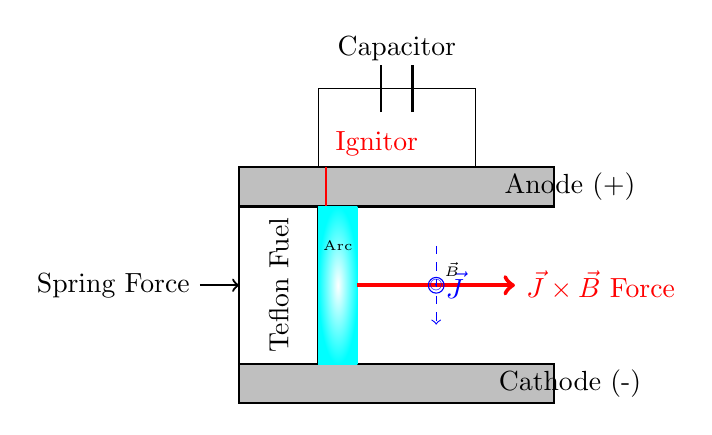
\begin{tikzpicture}
        % Electrodes
        \draw[thick, fill=gray!50] (0, 1) rectangle (4, 1.5); % Anode
        \draw[thick, fill=gray!50] (0, -1) rectangle (4, -1.5); % Cathode
        \node at (4.2, 1.25) {Anode (+)};
        \node at (4.2, -1.25) {Cathode (-)};
        
        % Teflon Fuel Bar
        \draw[thick, fill=white] (0, -1) rectangle (1, 1);
        \node at (0.5, 0) [rotate=90] {Teflon Fuel};
        \draw[->, thick] (-0.5, 0) -- (0, 0) node[pos=0, left] {Spring Force};
        
        % Capacitor Circuit
        \draw (1, 1.5) -- (1, 2.5) -- (3, 2.5) -- (3, 1.5);
        \draw (1, 2.5) -- (1.8, 2.5);
        \draw (2.2, 2.5) -- (3, 2.5);
        \draw[thick] (1.8, 2.2) -- (1.8, 2.8);
        \draw[thick] (2.2, 2.2) -- (2.2, 2.8);
        \node at (2, 3) {Capacitor};
        
        % Spark Plug
        \draw[thick, red] (1.1, 1.5) -- (1.1, 1.0);
        \node at (1.1, 1.8) [right, red] {Ignitor};
        
        % Plasma Discharge
        \shade[inner color=white, outer color=cyan] (1, -1) rectangle (1.5, 1);
        \node at (1.25, 0.5) {\tiny Arc};
        
        % Lorentz Force
        \draw[->, ultra thick, red] (1.5, 0) -- (3.5, 0) node[right] {$\vec{J} \times \vec{B}$ Force};
        \draw[->, blue, dashed] (2.5, 0.5) -- (2.5, -0.5) node[midway, right] {$\vec{J}$};
        \draw[blue] (2.5, 0) circle (0.1) node {\tiny $\odot$};
        \node at (2.7, 0.2) {\tiny $\vec{B}$};

    \end{tikzpicture}
    \caption{Electromagnetic: Pulsed Plasma Thruster (PPT)}
  \end{figure}
\end{frame}

\begin{frame}{Propellant Economics: The Shift from Xenon}
    \begin{table}
    \centering
    \begin{tabular}{l c c c}
        \toprule
        \textbf{Propellant} & \textbf{Mass (amu)} & \textbf{Cost} & \textbf{Use Case} \\
        \midrule
        \textbf{Xenon} & 131.3 & High ($\sim$\$3k/kg) & Science / GEO \\
        \textbf{Krypton} & 83.8 & Moderate & Starlink V1 \\
        \textbf{Argon} & 39.9 & Low ($\sim$\$10/kg) & Starlink V2 \\
        \textbf{Iodine} & 126.9 & Moderate & CubeSats (Solid) \\
        \bottomrule
    \end{tabular}
    \end{table}
    \vspace{0.2cm}
    \textbf{Starlink V2 (Argon):}
    \begin{itemize}
        \item 4.2 kW, $I_{sp} \approx 2500$ s.
        \item $\eta_T \approx 50\%$ (Lower than Xe, but economically viable).
        \item High ionization energy of Ar (15.8 eV) challenges efficiency.
    \end{itemize}
\end{frame}

\begin{frame}{Micro-Propulsion: Electrospray}
    \textbf{Physics:}
    \begin{itemize}
        \item Electrostatic extraction from liquid meniscus.
        \item \textbf{Taylor Cone} formation balance (Surface tension vs. Electric stress).
    \end{itemize}
    
    \begin{equation}
        V_{start} \approx \sqrt{\frac{\gamma r_c}{\epsilon_0}} \ln\left(\frac{4d}{r_c}\right)
    \end{equation}
    
    \textbf{Modes:}
    \begin{itemize}
        \item \textbf{Cone-Jet (Colloid):} Charged droplets.
        \item \textbf{Ionic (FEEP/ILIS):} Pure ion evaporation ($I_{sp} > 6000$ s).
    \end{itemize}
    \textbf{Scaling:} MEMS arrays (thousands of emitters) required for useful thrust.
\end{frame}

\begin{frame}{Electrospray Thruster Schematic}

  \begin{figure}[h]
    \centering
    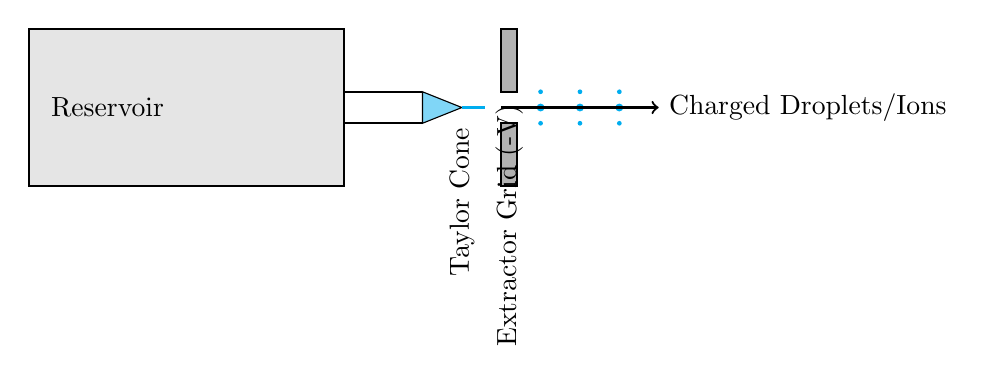
\begin{tikzpicture}[rotate=-90]
        % Emitter (rotated: originally vertical, now horizontal pointing right)
        \draw[thick, fill=gray!20] (0, 0) rectangle (2, 4);
        \node[rotate=0] at (1.0, 1.0) {Reservoir};
        
        % Capillary
        \draw[thick] (0.8, 4) -- (0.8, 5);
        \draw[thick] (1.2, 4) -- (1.2, 5);
        
        % Liquid / Taylor Cone
        \draw[fill=cyan!50] (0.8, 5) -- (1.0, 5.5) -- (1.2, 5) -- cycle;
        \node[rotate=90] at (2.2, 5.5) {Taylor Cone};
        
        % Extractor Grid
        \draw[thick, fill=gray!60] (0, 6) rectangle (0.8, 6.2);
        \draw[thick, fill=gray!60] (1.2, 6) rectangle (2, 6.2);
        \node[rotate=90] at (2.5, 6.1) {Extractor Grid (-V)};
        
        % Jet / Plume
        \draw[thick, cyan] (1.0, 5.5) -- (1.0, 5.8); % Jet
        \foreach \y in {6.5, 7, 7.5} {
            \fill[cyan] (1.0, \y) circle (0.05);
            \fill[cyan] (0.8, \y) circle (0.03);
            \fill[cyan] (1.2, \y) circle (0.03);
        }
        \draw[->, thick] (1.0, 6) -- (1.0, 8) node[rotate=0, right] {Charged Droplets/Ions};

    \end{tikzpicture}
    \caption{Micro-Propulsion: Electrospray Thruster}
  \end{figure}
\end{frame}

%---------------------------------------------------------
% Section 6: Conclusion
%---------------------------------------------------------
\subsection{Summary}

\begin{frame}{Conclusion}
    \begin{itemize}
        \item \textbf{Physics:} Power-limited rocket equation drives the design.
        \item \textbf{Technology Bifurcation:}
        \begin{itemize}
            \item \textbf{High Power/Life:} Magnetic Shielding enables Gateway/Mars (AEPS).
            \item \textbf{Low Cost/High Volume:} Argon Hall thrusters enable Mega-constellations (Starlink).
        \end{itemize}
        \item \textbf{Systems View:} PPU and Thermal management are dominant mass/volume drivers.
        \item \textbf{Future:} Higher power (100 kW+), alternative propellants (Iodine), and micro-scale integration.
    \end{itemize}
\end{frame}

\end{document}